\documentclass{thesisbyxetex}

\usepackage[xetex]{graphicx}	%	Подключаем графику
\usepackage{mathtools}		% 	Подключаем математические символы

\usepackage{amsmath}

\usepackage{fontspec}
\usepackage{unicode-math}
\usepackage{xunicode}
\usepackage{xltxtra}% говорят что не нужен

%для борьбы с переполнениями за счет разреженных слов в абзаце
\emergencystretch=25pt

\usepackage{polyglossia}
\setdefaultlanguage[spelling = modern]{russian}
\setotherlanguage{english} 
\defaultfontfeatures{Scale = MatchLowercase,Ligatures=TeX}  %% устанавливает поведение шрифтов по умолчанию  

\setmainfont{XITS}
\setmathfont{XITS Math}
\newfontfamily\cyrillicfont{XITS}
\setsansfont[Mapping=tex-text]{Nimbus Sans L}
\setmonofont{Nimbus Mono L}



\usepackage{enumitem}	
\setlist{nolistsep}	% отступы между элементами перечесления

\usepackage[unicode, pdfborder={0 0 0 0}]{hyperref}

\usepackage[autostyle]{csquotes}
\usepackage[%parentracker=true,
  backend=biber,
  hyperref=auto,
  language=auto,
  autolang=other,
  style=gost-numeric,
]{biblatex}
\addbibresource{bibliography.bib}

\begin{document}

\hypersetup{
pdftitle = {Курсовая работа},
pdfauthor = {Степанищев Артём Эдуардович},
pdfsubject = {курсовая},
pdfkeywords = {физический движок, язык D, курсовая}
}% End of hypersetup

\input{./Title/Title}	% Титульный лист
\tableofcontents 	% Оглавление, которое генерируется автоматически
\chapter*{Введение}	%	Пишем "Введение" вместо  "Глава 1 Введение"
\addcontentsline{toc}{chapter}{Введение}	%	Добавляем "Введение" в оглавление
Физический движок (англ. \textit{physics engine}) --- компьютерная программа, которая производит
компьютерное моделирование физических законов реального мира в виртуальном мире,
с той или иной степенью аппроксимации. Чаще всего физические движки используются не как отдельные 
самостоятельные программные продукты, а как составные компоненты (подпрограммы) других программ.

% TODO актуальность

Целью данной работы является написание библиотеки, моделирующей поведение твердых тел в трехмерном пространстве. 
Такая библиотека позволит разработчикам создавать приложения на основе физики твердого тела как в трехмерном, так и 
в двумерном пространстве. Такими приложениями могут является компьютерный игры.

Для достижение поставленной цели необходимо решить следующие задачи:%они мне не до конца нравятся
\begin{itemize}
  \item Рассмотреть и изучить законы изменения импульса, скорости и ускорения тела для моделирования
  движения тела в пространстве, законы изменения тензора инерции, угловой скорости и углового ускорения 
  для моделирования вращения тела в пространстве вокруг оси вращения.

  \item Рассмотреть особенности пересечений элементарных геометрических тел --- поскольку любое физическое тело обладает 
  геометрической формой, которую нельзя игнорировать при моделировании физических процессов.

  \item Рассмотреть основные способы интегрирования дифференциальных уравнений в рамках дисциплины численных методов, 
  позволяющие определить основные физические характеристики тела в момент времени.
\end{itemize}

% и мне совершенно не нравятся как написаны эти два абзаца
В качестве референтного языка используется язык программирования D.
Данный язык является из семейства языков программирования "фигурных скобок"
поэтому представленный в приложениях код будет интуитивно понятен читателю,
владеющему знаниями языка программирования С/С++ или Java.

Язык программирования D был выбран в связи с мощной реализацией шаблонов,
объемной стандартной библиотекой, а так же с быстротой работы.
Язык программирования D имеет широкое распространение от программного обеспечения веб-серверов
до бизнес решений и интернет приложений. 
\chapter{Моделирование динамики твердого тела}
\section{Типичные задачи для моделирования в компьютерных играх}

Компьютерные игры моделирует определенную окружающую среду,
называемую также игровым миром, в котором игровые объекты подчиняются
некоторым законам так, чтобы их поведение было ожидаемым и предсказуемым
для игрока. Для большинства игр основной интерес представляют передвижение
различных тел в пространстве, а также ряд визуальных феноменов механического
плана. Примерами таких игр являются: трилогия <<Crysis>>, серия игр <<FlatOut>>, <<Grand Theft Auto>> и другие.
Существуют игры из жанра головоломок (например, серия <<The incrdible machines>>, <<Auditorium>>, <<Zuma>> и т.д.)
), которые моделируют не только механические явления, однако они составляют
сравнительно малую часть всех игр.

% \/ Не знаю как согласовать это с введением, если выкинуть определение физ.движка из введенеия,
% \/ то оно вооще станет пустым :(
%Та часть компьютерной программы, которая отвечает за моделирования
%различных физических явлений в игровом мире получила устойчивое
%название physics engine --- физический движок (этим жаргонизмом ставшим термином мы и
%будем пользоваться в дальнейшем). Как было рассмотрено выше физический
%движок моделирует в основном механические явления. Наибольшее распространение и 
%значимость для компьютерных игр имеют следующие задачи:
%\begin{itemize}
% \item моделирование движения в поле консервативных сил (например, в гравитационном),
% \item моделирование столкновений тел (здесь рассматриваются как абсолютно упругие так и эластичные тела),
% \item моделирование сочленений и соединений,
% \item моделирование потоков воды, дыма, огня, которое обычно осуществляется системой частиц,
% \item моделирование тканей.
%\end{itemize}
%TODO здесь возможно стоит подробно пройтись по каждой задаче, а также оговорить, что реализовано, а что только будет реализовано


%\/ Частично описано в ведение, стот ли переносить что-то сюда?
%TODO нужно расказать об особенностях игровой физики: большое число объектов, realtime, визуальное, а не физическое подобие. 

\section{Физико-математическое описание механического движения}
Конечного пользователя интересует визуальное поведение игровых объектов.
Оно определяется положением тел в пространстве и времени и изучается кинематикой. Однако
кинематика не рассматривает причины возникновения движения --- этим занимается динамика. Поэтому
моделирование игровой сцены строится в следующем порядке: моделируется динамика (т.е. взаимодействие тел), на
его основе строится кинематическое описание, которое непосредственно и видит игрок. Фактически
моделирование игровой физики сводится к решению соответствующей обратной задачи механики.

%  \/ ээээ....я не знаю, что здесь написать
% TODO добавить абзац о различных способах аналитического моделирование одних и тех же явлений: 
% силовая динамика, законы сохранения, принцип наименьшего действия

% Обосновать необходимость численного моделирования

% \/ так же нет идеи что псиать здесь о точке и упругом теле. 
% \/ А о твёрдом теле рассказывается ниже в сответствующей подсекции
% TODO добавить абзац о материальной точке, абсолютно твердом теле и упругом теле

\subsection{Кинематическое описание}
\subsubsection{Материальная точка}
Положение тела в пространстве в любой момент времени задается функцией радиус вектора от
времени, получившей исторически название уравнение движения:
\begin{equation}
 \mathbf{r}=\mathbf{r}(t).
\end{equation}

Непосредственный вид уравнения движения может быть задан лишь в ограниченном числе 
тривиальных случаев. В реальных же задачах мы можем получить на основе динамики 
дифференциальное уравнение (или систему в случае многих тел), решением которого
будет искомое уравнение движения.
\begin{equation}
 \ddot{\mathbf{r}}=f(t, \mathbf{r}(t), \dot{\mathbf{r}}(t)).
\end{equation}

Первой и второй производной является скорость и ускорение соответственно.
Так как механическое состояние системы полностью характеризуется заданием координат
и скоростей \cite[10]{Landau1}, то возможны уравнения не выше второго порядка. 
В данном случае, скорость и ускорение --- величины векторные, поскольку они имеют величину и направление.

\subsubsection{Твердое тело}
Лишь некоторые тела могут быть промоделированы заданием лишь одного положения в пространстве 
(например, материальная точка), большинство тел имеет форму и по разному ведут себя в зависимости
от ориентации в пространстве. Существует несколько способов задания ориентации тела в трехмерном
пространстве. Изменение положения тела в пространстве характеризуются двумя псевдовекторами ---
угловой скоростью и угловым ускорением.
\subsubsection{Углы Эйлера}
% \/ попытался
%TODO здесь толком описать углы Эйлера (желательно с картинками) и проблему шарнирного замка
Углы Эйлера --- углы, описывающие поворот абсолютно твердого тела в трехмерном евклидовом пространстве.

Углы Эйлера определяют три поворота системы, которые позволяют привести любое положение системы к текущему.
Обозначим начальную систему координат как ($x$, $y$, $z$), конечную как ($X$, $Y$, $Z$).
Пересечение координатных плоскостей $xy$ и $XY$ называется линией узлов $N$.
\begin{itemize}
  \item Угол $\alpha$ между осью $x$ и линией узлов --- угол прецессии.
  \item Угол $\beta$ между осями $z$ и $Z$ --- угол нутации.
  \item Угол $\gamma$ между осью $X$ и линией узлов --- угол собственного вращения.
\end{itemize}
  
Повороты системы на эти углы называются прецессия, нутация и поворот на собственный угол (вращение).
Такие повороты некоммутативны и конечное положение системы зависит от порядка, в котором совершаются повороты. 

\begin{figure}[ht!]
\begin{center}
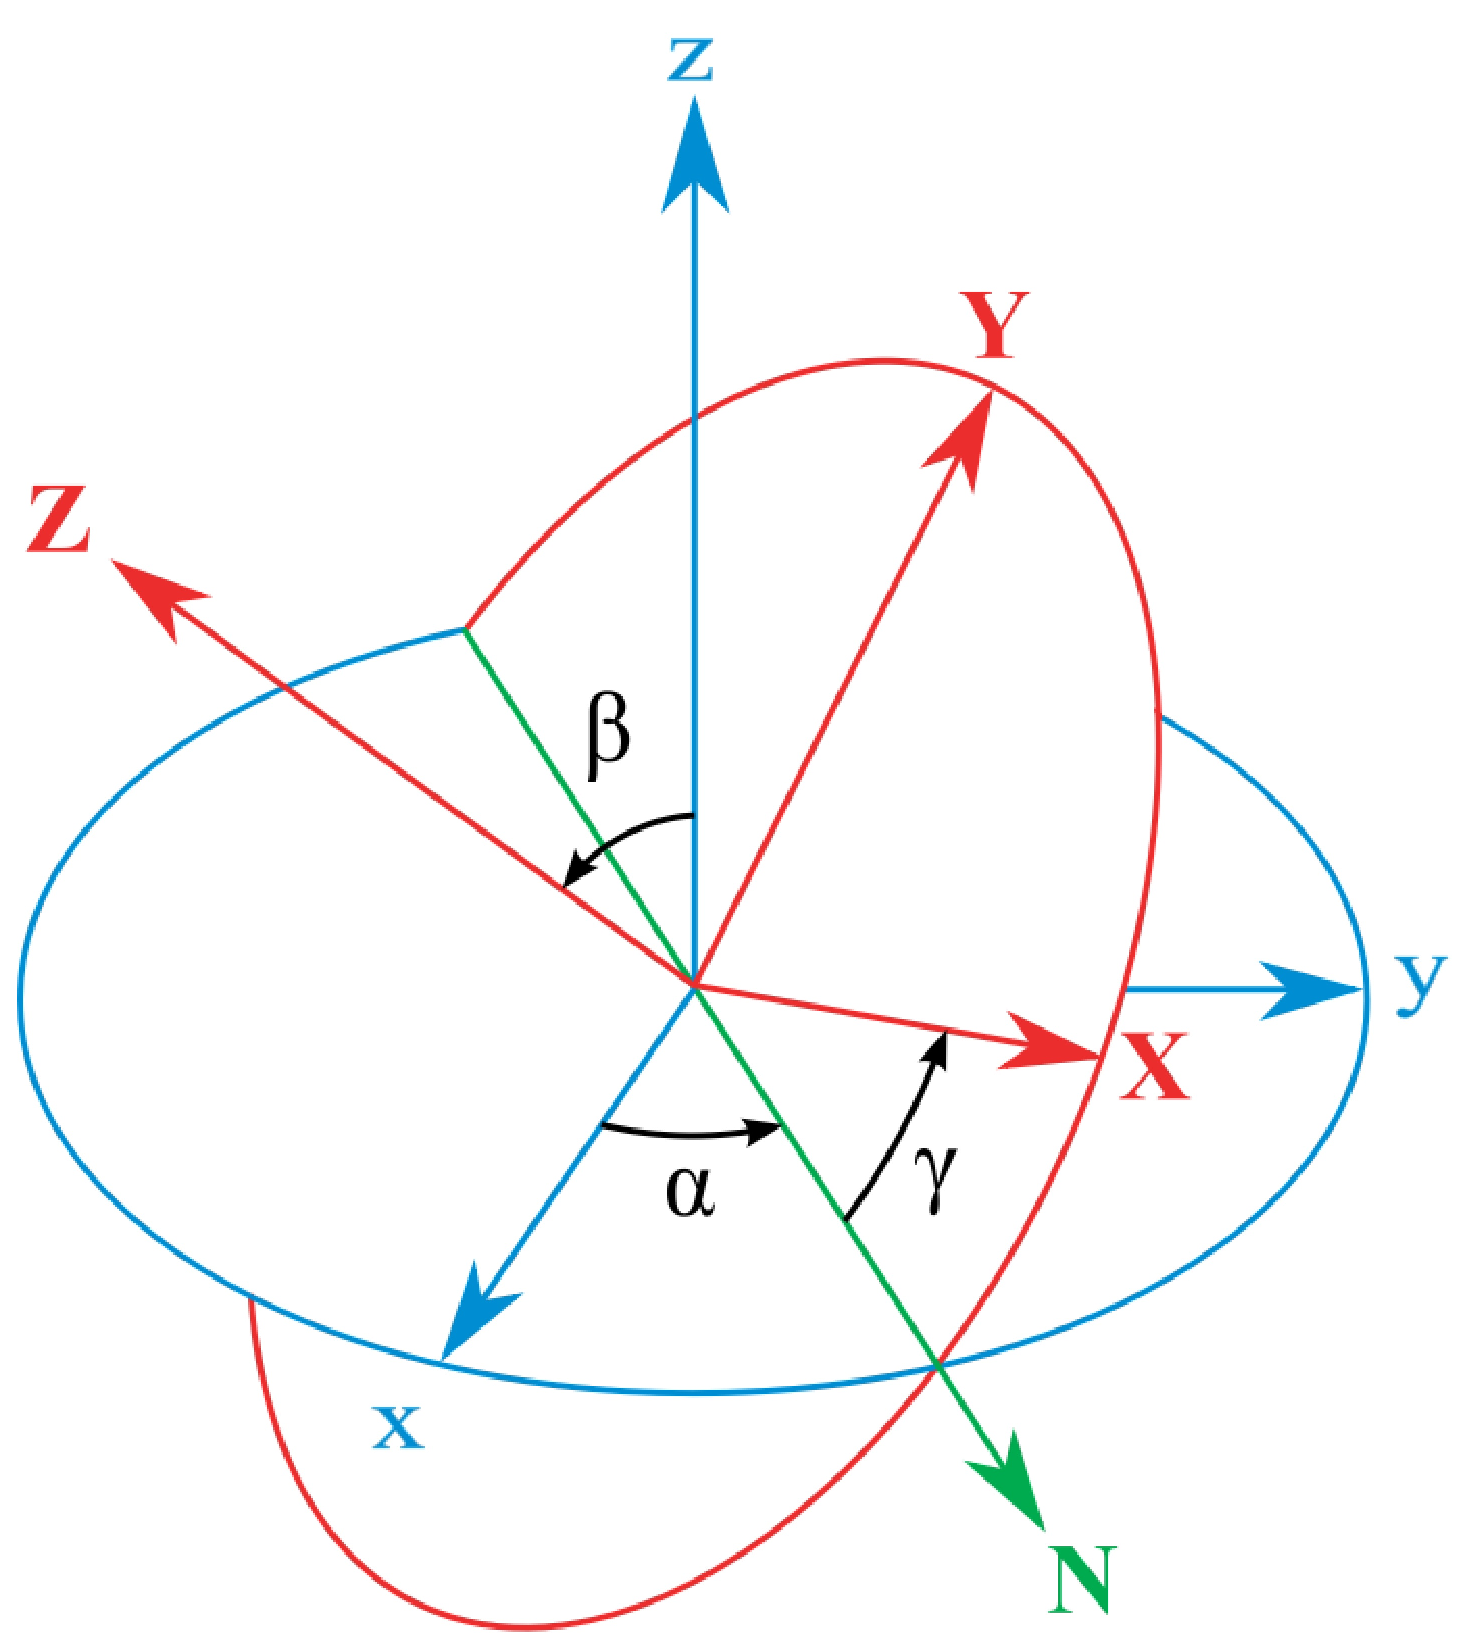
\includegraphics[scale=0.25]{./Rigidbody/Eulerangles.eps}  \\
\caption{Углы Эйлера}\label{Eulerangles}
\end{center}
\end{figure}

\subsubsection{Матрица поворота}
% \/  ...попытался
%TODO описать матрицу поворота
Матрицей поворота (или матрицей направляющих косинусов) называется ортогональная матрица,
которая используется для выполнения собственного ортогонального преобразования в евклидовом пространстве.
При умножении любого вектора на матрицу поворота длина вектора сохраняется. Определитель матрицы поворота равен единице.
Обычно считают, что, в отличие от матрицы перехода при повороте системы координат (базиса),
при умножении на матрицу поворота вектора-столбца координаты вектора преобразуются в соответствии с поворотом
самого вектора (а не поворотом координатных осей; то есть при этом координаты повернутого вектора получаются в той же,
неподвижной системе координат). Однако отличие той и другой матрицы лишь в знаке угла поворота,
и одна может быть получена из другой заменой угла поворота на противоположный; та и другая взаимно обратны и могут быть получены
друг из друга транспонированием.

Любое вращение в трехмерном пространстве может быть представлено как композиция поворотов вокруг
трех ортогональных осей (например, вокруг осей декартовых координат).
Этой композиции соответствует матрица, равная произведению соответствующих трех матриц поворота.
Матрицами вращения вокруг оси декартовой системы координат на угол $\alpha$ в трехмерном пространстве являются:
\begin{itemize}
  \item Вращение вокруг оси $x$:
  \begin{equation}
    M_x(\alpha) = \begin{pmatrix} 
		  1 & 0          & 0           \\
		  0 & \cos\alpha & -\sin\alpha \\
		  0 & \sin\alpha & \cos\alpha
		  \end{pmatrix},
  \end{equation}
  
  \item Вращение вокруг оси $y$:
  \begin{equation}  
    M_y(\alpha) = \begin{pmatrix} 
		  \cos\alpha  & 0 & \sin\alpha \\
		  0          & 1 & 0           \\
		 -\sin\alpha & 0 & \cos\alpha
		  \end{pmatrix},
  \end{equation}
  \item Вращение вокруг оси $z$:
  \begin{equation}
    M_z(\alpha) = \begin{pmatrix} 
		  \cos\alpha & -\sin\alpha & 0 \\
		  \sin\alpha & \cos\alpha  & 0 \\
		  0          & 0           & 1
		  \end{pmatrix}.
  \end{equation}
\end{itemize}
Во всех примерах приведены матрица поворота от результирующей системы координат к исходной.
  
\subsubsection{Кватернион}
% \/  ...попытался
%TODO описать кватернион и его связь с поворотом и угловой скоростью
Кватернионы предоставляют удобное математическое обозначение положения и вращения объектов в пространстве.
В сравнении с углами Эйлера, кватернионы позволяют проще комбинировать вращения, а также избежать проблемы,
связанной с невозможностью поворота вокруг оси, независимо от совершенного вращения по другим осям.
В сравнении с матрицами они обладают большей вычислительной устойчивостью и могут быть более эффективными.
Кватернионы нашли свое применение в компьютерной графике, робототехнике, навигации, молекулярной динамике.

Кватернион выгодно использовать в компьютерных вычислениях, так как представление кватерниона требует
лишь 4 компоненты, против 9 компонент (3 вектора по 3 компоненты) у углов Эйлера и 9 компонент у матрицы поворота.

\subsection{Динамическое описание}
Согласно силовой модели механики равнодействующая сил приложенных к телу вызывает ускорение (второй закон Ньютона)
\begin{equation}
 \mathbf{a}=\frac{\sum\limits_{i=1}^n{\mathbf{F}_i}}{m}.
\end{equation}
Всего существует только четыре природы силовых взаимодействий: гравитационная, электромагнитная, сильная и слабая.
Последние две проявляют себя только на микроуровне, поэтому их нет необходимости рассматривать в задачах
игровой физики. Гравитационная природа представлена полем тяготения, которое является консервативным. 
Все остальные силы являются проявлением взаимодействий электромагнитной природы на микро и макроуровне.
Однако оказывается весьма неудобным при рассмотрении макроявлений использовать электромагнитные силы на микроуровне,
поэтому вводятся макрообощения характеризующее соответствующее явление в целом, например, закон Кулона
для трения или закон Гука для упругости.

Во многих случаях даже такое макроописание является слишком подробным и сложно реализуемым на компьютере,
поэтому часто моделируют только абсолютно твердые тела, для взаимодействия которых выполняется закон 
сохранения импульса.
\subsubsection{Динамика вращательного движения}
Для вращательного движения тела можно ввести ряд характеристик
являющимися аналогами уже рассмотренных для поступательного движения.
Радиус вектору $ \mathbf{r} $ соответствует кватернион $q$ или матрица вращения $\mathrm{R}$,
скорости $\mathbf{v}$ --- угловая скорость $\boldsymbol{\omega}$ направленная вдоль оси вращения,
ускорению $\mathbf{a}$ --- $\boldsymbol{\alpha}$ угловое ускорение.
Вызванное силой вращение зависит не только от силы, но и от положения точки приложения силы
по отношению к мгновенному центру вращения, величина аналогичная силе носит название момента силы:
\begin{equation}
 \mathbf{M} = \mathbf{r}\times{\mathbf{F}}, 
\end{equation}
она также как и сила является аддитивной величиной.

Мера отклика на момент силы зависит не только от массы тела, но и от геометрии распределения
масс в теле. Данная величина получила название момента инерции тела:
\begin{equation}
 J=\int\limits_{V} \rho r^2\mathrm{d}V.
\end{equation}

В общем случае момент инерции зависит от направления оси вращения и поэтому является тензорной
величиной $\mathrm{J}$ (фактически двухмерной матрицей \begin{math}3\times3\end{math}), компоненты которого могут
быть выражены как:
\begin{equation}
 \mathrm{J}_{ij} = \int\limits_{V} (\delta_{ij}r^2 - \mathbf{r}_i \mathbf{r}_j) \rho \mathrm{d}V,
\end{equation}
где $\delta_{ij}$ символ Кронекера, а $\mathbf{r}$ радиус-вектор из центра вращения к точке интегрирования.
Тензор инерции всегда является положительно определенным и может быть приведен к диагональному виду. Момент
инерции относительно произвольно расположенной оси вращения может быть выражен через момент инерции параллельной
оси вращения проходящей через центр масс по теореме Гюйгенса--Штейнера:
\begin{equation}
 J=J_C+md^2.
\end{equation}

%TODO Дать формулу связывающую момент силы, момент инерции и угловое ускорение в случае, 
% когда момент инерции является тензорной величиной. (я пока нашёл лишь через кососимметричные матрицы) 
% также в обязательном порядке дать корректные формулировки связи кватерниона и угловой скорости
%\begin{equation}
%q = \frac{1}{2}q_0\omega{\delta{t}} 
%\end{equation}

% Возможно нужно что-то ещё, но собственно это резюме этой части
Таким образом, динамическое тело может быть описано
следующими минимальными характеристиками:
\begin{itemize}
  \item масса (скаляр)
  \item позиция (вектор)
  \item скорость (вектор)
  \item ускорение (вектор) %???
  \item сумма сил (вектор) %???
  \item момент инерции (матрица)
  \item поворот (кватернион)
  \item угловая скорость (вектор)
  \item угловое ускорение (вектор) %???
  \item сумма моментов сил (вектор) %???
\end{itemize}
% величины отмеченные вопросом на мой взгляд являются вычислимыми или внешними величинами
% поэтому нужно ли их хранить в объекте (это касается не только текста, но и вашего кода).

% TODO это надо переформулировать и обосновать (что за ``не любит'', у этого есть математические обоснования)
% также нужно подумать где это расположить
%
%В любой момент времени скорость тела зависит от
%времени, прошедшего между двумя шагами симуляции – \begin{math}\Delta\end{math}t. Это
%время, как правило, фиксировано и должно соответствовать
%времени между двумя кадрами рендеринга – например, 1/60 с.
%
%Это соответствует 60 кадрам в секунду, как в системах с
%включенной вертикальной синхронизацией.
%В кинематике (идеализированном описании движения) в
%качестве \begin{math}\alpha\end{math} часто берется реальное время между кадрами, но
%динамика такой подход «не любит»: при резких скачках \begin{math}\alpha\end{math}
%(например, вследствие запоздания графики), тела
%приобретают неестественно большие скорости и начинают
%пролетать сквозь препятствия.

\chapter{Геометрия твердых тел}
\section{Геометрические примитивы}
Описание движения тела полностью абстрагировано от его формы
или, как принято выражаться, геометрии --- это очень важно
уяснить для понимания внутренней архитектуры физического
движка.

Основными геометрическими примитивами используемыми в физических движках являются:
\begin{itemize}
 \item  луч, 
 \item  плоскость,
 \item  полигон,
 \item  сфера,
 \item  треугольник
 \end{itemize}
Для реализации более сложных геометрических тел используется композиция тел представленных выше.

Рассмотрим более подробно один основных из геометрических примитивов --- сферу.
Сфера может быть описана в пространстве положением своего геометрического цента(он же является и центром масс)
и радиуса. Таким образом для описания сферы достаточно 4 компонент : вектора положения центра сферы( 3 компоненты) и радиуса сферы.

%TODO Рассмотреть большее количество геометрически примитивов

\section{Контакт геометрических тел}
Реализации твердого тела и геометрического объекта как правило раздельны --- геометрия тела играет роль только в
процессе обнаружения столкновений, рассматриваемый ниже.

Модули обнаружения столкновений (\textit{collision detection}) и реагирования на столкновения (\textit{collision responce}) представляют 
собой ключевые компоненты любого физического движка. Именно они в процессе симуляции осуществляют главную нагрузку на
процессор, и именно от них требуется максимальная точность.

\subsection{Обнаружение столкновений}
Методы обнаружения столкновений подразделяются на две категории: статические и динамические. В первом случае
движение тел рассматривается как последовательность «квантовых скачков» --- проверка на пересечение двух геометрий
производится в промежутках между скачками, как если бы объекты в этом время не двигались (то есть, имели нулевые
скорости). Основным допущением этого метода является временная когерентность системы --- предполагается, что тела
обладают небольшими скоростями, и их позиции не меняются слишком резко с течением времени. Иными словами,
статическое обнаружение столкновений плохо подходит для моделирования, например, пушки, стреляющей в бетонную
стену: за шаг времени ($\Delta{t}$) снаряд пройдет расстояние, значительно превышающее толщину стены, и, следовательно,
попросту пролетит сквозь нее --- статическая проверка это столкновение не обнаружит.

Динамическое обнаружение столкновений\cite{Ericson} использует другой метод, при котором учитывается скорость тела --- движок
предсказывает, какое положение в пространстве займет объект на следующем шаге времени, если будет двигаться с той же
скоростью. Фактически, делается проверка на пересечение отрезка, представляющего собой траекторию движения тела, с
препятствием --- вычисляется точка, в которой тело столкнется с этим препятствием, и на основании этой информации движок
делает соответствующие корректировки. К сожалению, динамический метод довольно сложен (особенно для
нетривиальных геометрий) и, в целом, плохо адаптирован для динамики как таковой --- он чаще используется в кинематике.
Поэтому далее будет рассматриваться статический метода --- он, при всех его недостатках, хорошо себя оправдывает в
большинстве физических ситуаций.

В физическом движке функция проверки столкновения между двумя объектами должна давать на выходе следующую
информацию:
\begin{itemize}
  \item точка контакта
  \item вектор нормали к поверхности столкновения в этой точке (нормаль контакта)
  \item глубина взаимного проникновения объектов
\end{itemize}

\begin{figure}[ht!]
\begin{center}
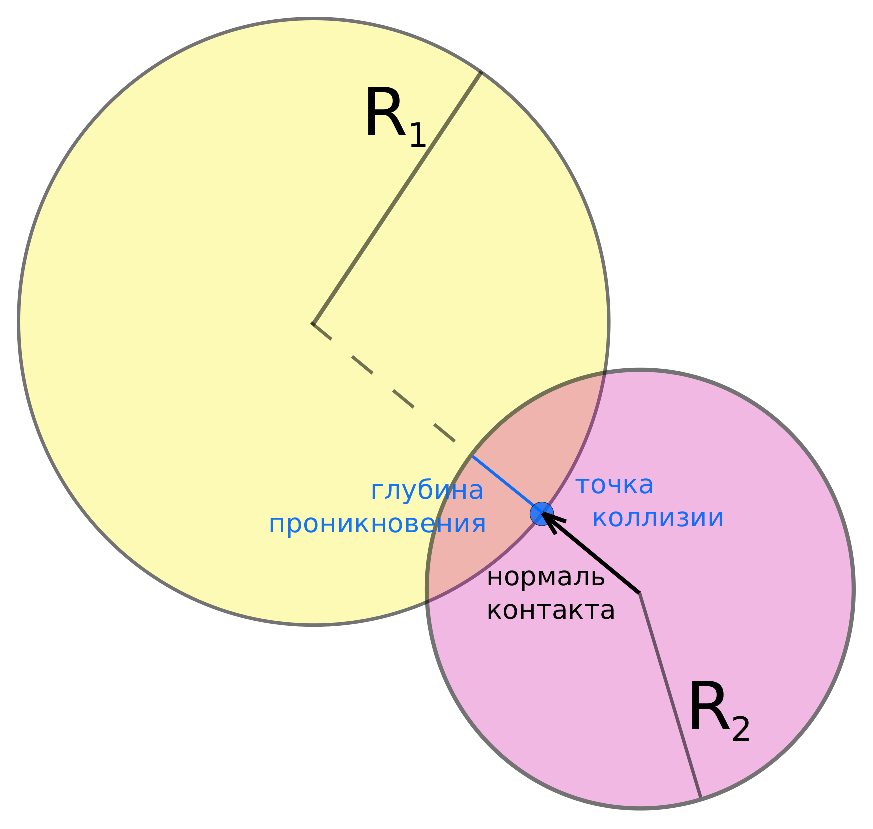
\includegraphics[scale=0.45]{./Geometry/SphereCollision.eps} \\
\caption{Контакт двух сфер}\label{SphereCollision} 
\end{center}
\end{figure}
Эти три свойства, вкупе со ссылками на столкнувшиеся тела, дают новую сущность --- контакт. Соответственно,
процесс обнаружения столкновений в терминологии физического движка также называют генерированием
контактов (\textit{contact generation}). В сложных движках на одно столкновение между двумя телами приходится несколько
контактов --- так называемый \textit{contact manifold}. Далее будет рассматриваться простейший случай --- столкновение сфер, где будет
достаточно одного контакта на пару столкнувшихся тел.

Рассмотрим одно очевидным свойство. Если сумма радиусов двух сфер превышает расстояние между их центрами, следовательно, сферы пересекаются.
При этом нормаль столкновения --- это нормированный вектор от центра второй сферы в сторону центра первой,
точка столкновения --- экстремальная точка на поверхности второй сферы в направлении этого вектора, а глубина взаимного
проникновения --- разница между суммой радиусов и расстоянием (см. рисунок \ref{SphereCollision}). % здесь ссылка возможно 
% и не нужна, вставил для пробы

Таким образом можно легко обнаружить столкновение таких двух примитивов как сферы.
\subsection{Реагирование на столкновение}
Получив необходимую информацию о контакте(точку контакта, нормаль контакта и глубину проникновения), модулю реагирования
на столкновения необходимо скоординировать скорости тел таким образом, чтобы тела перестали пересекаться и проникать друг в друга.  

При моделировании используются алгоритм отличный от реального поведения: объекты выталкиваются вдоль вектора нормали на величину,
равную половине глубины взаимопроникновения:

\begin{equation}
\mathbf{x} = \frac{1}{2}\mathbf{x}_0 + d\mathbf{n}
\end{equation}
\begin{eqrem}
$\mathbf{x}_0$ --- точка контакта,

$d$ --- глубина взаимопроникновения,

$\mathbf{n}$ --- вектор нормали контакта.
\end{eqrem}

Первый объект выталкивается вдоль $+\mathbf{n}$, а второй – вдоль $-\mathbf{n}$ (вектор нормали контакта указывает от второго тела к первому).

Эту операцию называют также корректировкой позиций (\textit{position correction}). Но такой подход нестабилен, кроме того,
необходимо учитывать массы тел и, следовательно, импульс.

Импульс – это векторная величина, мера механического движения тела. Вращательным аналогом импульса является момент импульса.
\begin{equation}
\mathbf{L} = \mathbf{r}\times\mathbf{p}
\end{equation}
\begin{eqrem}
$\mathbf{p}$ --- линейный импульс,

$\mathbf{r}$ --- радиус-вектор (точка, к которой приложен линейный импульс).
\end{eqrem}



\printbibliography
\addcontentsline{toc}{chapter}{Литература}

\end{document}